\documentclass[conference]{IEEEtran}
\IEEEoverridecommandlockouts
% The preceding line is only needed to identify funding in the first footnote. If that is unneeded, please comment it out.
%Template version as of 6/27/2024
\usepackage[utf8]{inputenc}
\usepackage[T1]{fontenc}
\usepackage[brazilian]{babel}
\usepackage{algorithm}
\usepackage{booktabs}
\usepackage{float}
\usepackage{algpseudocode}
\usepackage{cite}
\usepackage{amsmath,amssymb,amsfonts}
% \usepackage{algorithmic}
\usepackage{graphicx}
\usepackage{textcomp}
\usepackage{xcolor}
\def\BibTeX{{\rm B\kern-.05em{\sc i\kern-.025em b}\kern-.08em
    T\kern-.1667em\lower.7ex\hbox{E}\kern-.125emX}}
\begin{document}

\title{Modelos ocultos de Markov na detecção sequencial de respostas auditivas de estado estável: uma comparação com o teste de Rayleigh}

\author{\IEEEauthorblockN{1\textsuperscript{o} Victor Hugo de Souza Singulani Ragazzi}
\IEEEauthorblockA{\textit{Departamento de Engenharia Elétrica} \\
\textit{Universidade Federal de Viçosa}\\
Viçosa, Brasil \\
victor.ragazzi@ufv.br}
}

\maketitle

\begin{abstract}
Estratégias de detecção automática de uma resposta auditiva de estado estável (ASSR, do inglês \textit{auditory steady-state response}), podem ser realizadas a partir da aplicação de testes estatísticos o qual é comparado a um valor crítico. O objetivo deste trabalho é avaliar se um modelo oculto de Markov (HMM, do inglês \textit{Hidden Markov Model}) com dois estados ocultos, resposta ausente e resposta presente, supera a detecção quando a estatística do teste de Rayleigh é usada como sua observação. Em vez de uma matriz de observação discreta, cada estado é descrito por uma função densidade de probabilidade Gama, e a densidade do estado presente é obtida de um modelo bayesiano hierárquico amostrado por Monte Carlo via cadeias de Markov (MCMC). O método foi avaliado em registros de onze adultos, deixando um participante de fora por vez. Com cada registro analisado separadamente, o HMM obteve um taxa de detecção de 1.8\% menor que o teste de Rayleigh sozinho, com taxa de falsos positivos similares (8,3\% e 8,5\%), o tempo de detecção médio foi de 6 segundos \textbf{a menos} para o HMM, entretanto, nenhuma dessas diferenças foram significativa. Quando os registros de um participante foram analisados como uma única sequência, o HMM detectou 57,7\% contra 51,6\%, com taxa de falsos positivos nas frequências vizinhas de 8,0\% contra 6,1\%, diferença que não foi significativa. O HMM acrescenta pouco quando a observação já acumula a evidência do exame, e torna-se útil quando a informação pode ser transportada de um registro para o seguinte.
\end{abstract}

\begin{IEEEkeywords}
Eletroencefalograma, resposta auditiva de estado estável, testes sequenciais, modelo oculto de Markov, inferência bayesiana, falso positivo.
\end{IEEEkeywords}

\section{Introdução}

A avaliação auditiva é uma etapa crucial no diagnóstico e no tratamento de problemas de audição, especialmente em crianças. Segundo o Joint Committee on Infant Hearing \cite{jcih2007}, a avaliação auditiva é recomendada até o terceiro mês de vida, visando iniciar o tratamento o mais cedo possível em caso de risco de perda auditiva. A necessidade de agilizar a avaliação auditiva é importante para minimizar custos e prevenir dificuldades de audição.

Para crianças pequenas, bebês e indivíduos pouco cooperativos, recomenda-se o uso de audiometria objetiva, como as Emissões Otoacústicas (EOA) ou a Resposta Auditiva do Tronco Encefálico (ABR, do inglês \textit{Auditory Brainstem Response}) \cite{picton2003}. Dentre essas técnicas, a avaliação da Resposta Auditiva de Estado Estável (ASSR) surge como complemento às estratégias de ABR e EOA \cite{sturzebecher1999}. A ASSR permite estimar a audição em diferentes frequências simultaneamente, o que a torna particularmente útil para identificar perdas auditivas em frequências específicas \cite{sininger2018}. A resposta é um potencial evocado detectado no eletroencefalograma (EEG).

A detecção de ASSRs em sinais de EEG é conduzida por procedimentos estatísticos no domínio do tempo ou da frequência, conhecidos como Detectores Objetivos de Resposta (ORD, do inglês \textit{Objective Response Detectors}) \cite{sturzebecher1999}. O teste pode ser aplicado uma única vez ao final da coleta do EEG (\textit{Single-Shot}) ou realizado antes da coleta completa do sinal e repetido em intervalos de tempo definidos. Nessa estratégia de testes sequenciais, o processo se repete até identificar uma resposta ou atingir o limite de tempo, o que permite reduzir o tempo de detecção \cite{zanotelli2020,vaz2024,cebulla2015}. No entanto, a repetir a aplicação do teste aumenta a probabilidade de falsos positivos (FP), isto é, de detectar resposta em sinais sem resposta.

Nessas estratégias, cada aplicação do teste compara o valor corrente da estatística com um valor crítico, de forma independente das aplicações anteriores, a trajetória da estatística ao longo do exame não tem peso na decisão. Um Modelo Oculto de Markov (HMM) oferece uma forma de incorporar essa informação, o estado de interesse oculto, ausência ou presença de resposta, não é observado diretamente, mas gera uma sequência de observações, e a probabilidade de cada estado é inferida a partir de toda a sequência \cite{rabiner1989}

O objetivo deste trabalho é avaliar se o uso da estatística do teste de Rayleigh como observação de um HMM de dois estados melhora a taxa de detecção, ou encurta o tempo de detecção, em relação ao teste original, sem aumentar a taxa de FP. A matriz de observação do HMM é substituída por funções densidade de probabilidade, uma para cada estado, e a densidade do estado com resposta é estimada com um modelo bayesiano hierárquico.

\section{Fundamentação teórica}

Este trabalho combina duas ideias. Os detectores objetivos de resposta (ORDs) decidem se há uma ASSR comparando uma estatística com um valor crítico, obtido de uma distribuição de dados com resposta ausente. Os modelos ocultos de Markov (HMMs), por sua vez, inferem um estado não observável a partir de uma sequência de medidas. A primeira ideia fornece a estatística usada como observação; a segunda, a estrutura que permite aproveitar a evolução dessa estatística ao longo do exame.

\subsection{Detecção da ASSR}

Uma ASSR estimulada por um tom modulado na frequência $f_m$ aparece no espectro do EEG como uma componente em $f_m$, a qual, a fase se repete de uma época para a seguinte. Os ORDs no domínio da frequência testam essa regularidade usando a fase, a amplitude ou ambas \cite{dobie1993,sturzebecher1999,cebulla2006}. O teste de Rayleigh usa apenas a fase: sem resposta, as fases são uniformemente distribuídas e, com resposta, concentram-se em torno de uma direção preferencial \cite{mardia2000}.

Para a aplicação sequencial, Stürzebecher et al. \cite{sturzebecher2005} obtiveram por simulação um valor crítico constante que mantém a taxa de FP controlada. Outras estratégias acrescentam harmônicos superiores ao detector \cite{cebulla2006}, ouo um valor crítico que cresce a cada etapa do teste \cite{sturzebecher2013} e um intervalo variável entre os testes \cite{cebulla2015}. Outros autores propõe regras de parada baseadas no número de detecções consecutivas \cite{zanotelli2020} e critérios para interromper o exame quando não se espera resposta \cite{vaz2024}. Todas comparam uma estatística com um valor crítico calibrado sob a hipótese de ausência de resposta.

\subsection{Modelos ocultos de Markov}

Um HMM é definido pelas probabilidades iniciais dos estados $\pi$, pela matriz de transição de estados $A$ e pela distribuição de observação $B$ de cada estado \cite{rabiner1989}. Quando as observações são contínuas, $B$ é um conjunto de funções densidade de probabilidade em vez de uma matriz. Dada uma sequência de observações, o algoritmo de Viterbi encontra a sequência mais provável de estados ocultos \cite{viterbi1967}. HMMs têm sido aplicados ao EEG em problemas nos quais um estado dura por algum tempo, como a classificação \textit{online} de tentativas únicas em interfaces cérebro-computador \cite{obermaier2001}.

Na detecção da ASSR, o método mais próximo que encontrei é o uso de um filtro de Kalman, usado para estimar a amplitude e a fase da resposta ao longo do exame \cite{luke2017}. Buscando na literatura, não foi encontrado nenhum estudo que aplique um HMM à detecção da ASSR.

\section{Metodologia}

O método tem três partes: a observação, que utiliza 10 épocas do EEG para gerar um valor produzido pelo ORD; o HMM, que descreve como essa observação se comporta quando a resposta está ausente e quando está presente; e a regra de decisão, que transforma a sequência de estados inferidos em uma detecção ou não. A observação é a mesma para o HMM e para o teste de Rayleigh. Assim, a diferença entre os dois vem apenas de como a sequência de valores dos testes é interpretada.

\subsection{Observação: estatística de Rayleigh acumulada}

O EEG é dividido em épocas de um segundo e a transformada de Fourier de cada época fornece a fase $\theta_i$ na frequência de modulação. Com $N$ épocas coletadas, o teste de Rayleigh é
\begin{align}
Z_N &= N R^2; \qquad R=\sqrt{C^2+S^2}; \label{eq:z}\\
C &= \frac{1}{N}\sum_{i=1}^{N}\cos\theta_i; \qquad
S = \frac{1}{N}\sum_{i=1}^{N}\sin\theta_i .
\end{align}
Sem resposta, as fases são uniformes e independentes, de modo que $E[Z_N]=1$ e, para $N$ moderado ou grande, $Z_N$ segue aproximadamente uma distribuição exponencial de média um, o valor-p é então $p\approx e^{-Z_N}$ \cite{mardia2000}. Com resposta, as fases têm uma direção preferencial e o valor esperado do teste cresce com o número de épocas:
\begin{equation}
E[Z_N]=1+(N-1)\rho ,
\label{eq:media}
\end{equation}
em que $\rho$, entre 0 e 1, é o comprimento quadrático do vetor médio de fase e mede a força da resposta.

A estatística é recalculada a cada $M_{step}=10$ novas épocas, sempre com todas as épocas coletadas desde o início. A sequência $Z_{10}, Z_{20}, Z_{30},\ldots$ é a observação tanto do teste de Rayleigh quanto do HMM.

O uso do teste de Rayleigh como observação não é uma exigência do método: outros ORDs podem ser usados no lugar de $Z_N$, desde que convertidos para a mesma escala. Uma ablação com outros quatro ORDs é apresentada no Apêndice~\ref{app:ords}.


\subsection{HMM com funções densidade como modelo de observação}

O HMM tem dois estados ocultos, resposta Ausente ($\mathcal{A}$) e resposta Presente ($\mathcal{P}$), uma probabilidade inicial $\pi$ do estado Presente e uma matriz de transição $A$ de dimensão $2\times2$. Cada estado tem uma densidade Gama, escrita aqui com forma $k$ e média $\mu$:
\begin{align}
b_{\mathcal{A}}(z) &= \mathrm{Gama}(z \mid k_0,\ \mu_0), \label{eq:aus}\\
b_{\mathcal{P}}(z \mid N) &= \mathrm{Gama}\big(z \mid k,\ 1+(N-1)\rho\big). \label{eq:pres}
\end{align}
A família Gama contém a distribuição exponencial esperada sem resposta. Assumindo que a densidade Ausente é estática, utiliza-se os dados coletados \textbf{sem estimulação} para calcular a máxima verossimilhança, encontrando um $k_0$ e $\mu_0$ que representem melhor os dados. A densidade Presente vai deslocando para a direita à medida que o exame avança, seguindo \eqref{eq:media}.

\begin{figure*}[t]
\centering
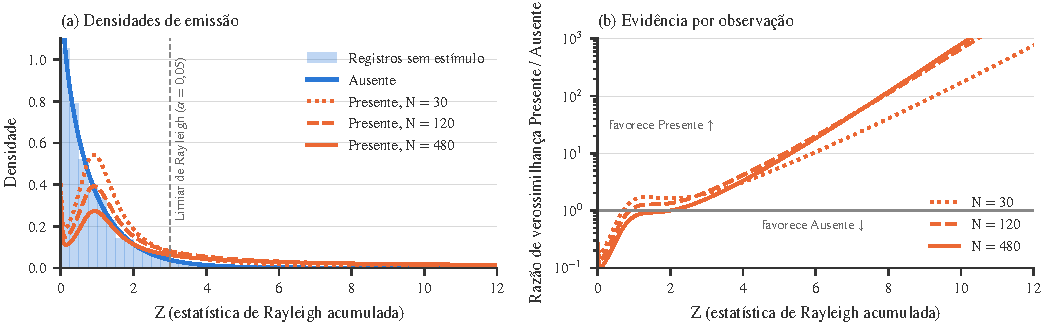
\includegraphics[width=0.8\textwidth]{figuras/fig_emissoes_pt.pdf}
\caption{Modelo de observação do HMM, ajustado com todos os participantes. (a) Densidade de cada estado; o histograma mostra os valores de $Z$ nos registros sem estimulação, e a densidade Presente é desenhada para três números de épocas $N$. (b) Razão entre as densidades Presente e Ausente, em escala logarítmica.}
\label{fig:emissoes}
\end{figure*}

\subsection{Modelo bayesiano hierárquico do estado Presente}

A resposta não tem a mesma força em todos os exames. Em vez de fixar $k$ e $\rho$, cada sequência de calibração $s$ tem seu próprio par $(k_s,\rho_s)$, sorteado de distribuições populacionais:
\begin{equation}
\begin{aligned}
Z_{s,t}\mid k_s,\rho_s &\sim \mathrm{Gama}\big(k_s,\ 1+(N_{s,t}-1)\rho_s\big),\\
k_s \sim \mathrm{Gama}&(a_k,b_k),\qquad \rho_s \sim \mathrm{Gama}(a_\rho,b_\rho),
\end{aligned}
\label{eq:hier}
\end{equation}
com forma $a$ e taxa $b$. Os quatro hiperparâmetros recebem uma distribuição \textit{a priori} uniforme, $p(a)\propto 1/a$.

A distribuição \textit{a posteriori} conjunta dos hiperparâmetros e de todos os pares $(k_s,\rho_s)$ não tem forma fechada e foi amostrada por Monte Carlo via cadeias de Markov (MCMC) \cite{gelman2013}. As taxas $b_k$ e $b_\rho$ têm condicionais completas Gama e foram sorteadas por amostragem de Gibbs; os demais parâmetros foram atualizados por passos de Metropolis com passeio aleatório na escala logarítmica. Quatro cadeias foram executadas por 20\,000 iterações, descartando-se as primeiras 5\,000 e mantendo-se uma a cada dez das restantes. A convergência foi verificada com a estatística $\hat{R}$ \cite{gelman1992}, e os diagnósticos completos de todas as rodadas de validação são apresentados no Apêndice~\ref{app:mcmc}.

A densidade usada pelo HMM é a densidade preditiva \textit{a posteriori} de um novo exame. Para cada uma de $M=2000$ amostras da distribuição \textit{a posteriori} dos hiperparâmetros, sorteia-se um par $(k_m,\rho_m)$ de \eqref{eq:hier}, e
\begin{equation}
b_{\mathcal{P}}(z\mid N)\approx\frac{1}{M}\sum_{m=1}^{M}\mathrm{Gama}\big(z\mid k_m,\ 1+(N-1)\rho_m\big).
\label{eq:pred}
\end{equation}

% Nada é aprendido durante o exame: após a calibração, \eqref{eq:aus} e \eqref{eq:pred} são curvas fixas.

\subsection{Decisão}

A cada avaliação $t$, o algoritmo de Viterbi é aplicado às observações coletadas até o momento, $Z_{10},\ldots,Z_{10t}$, combinando $\pi$, $A$ e as duas densidades. A avaliação é contada como positiva se a sequência de estados mais provável contém o estado Presente. Para o teste de Rayleigh, a avaliação é positiva se $Z_n\ge\alpha$.

O exame é interrompido, com uma detecção, na primeira avaliação em que uma regra de parada é satisfeita. As regras consideradas exigem um número mínimo de avaliações positivas consecutivas, uma fração mínima de avaliações positivas até o momento, ou uma combinação de ambos (144 regras). Nenhuma regra pode interromper o exame antes da terceira avaliação (30 s).

\section{Experimentos}

Os detectores foram avaliados em registros reais de EEG de onze adultos com audição normal. Espera-se resposta em todos os registros estimulados, enquanto nos registros sem estimulação  (ESP) ou nas frequências vizinhas, esperasse a ausência de resposta. Dessa forma, é medida a taxa de detecção e a taxa de FP.

\subsection{Dados}

Onze indivíduos adultos participaram do estudo, sendo duas mulheres e nove homens, com audição considerada normal. As frequências portadoras para ambas as orelhas foram as mesmas: 500, 1000, 2000 e 4000 Hz, moduladas respectivamente em 81, 85, 89 e 93 Hz para a orelha direita e 83, 87, 91 e 95 Hz para a orelha esquerda. A pesquisa recebeu aprovação do Comitê de Ética local (CEP/UFV nº 2.105.334), e todos os voluntários assinaram um termo de consentimento livre e esclarecido. A coleta de dados ocorreu em cabine acusticamente isolada. O EEG foi adquirido com dezesseis eletrodos dispostos segundo o Sistema Internacional 10-20 (apenas o eletrodo FC foi analisado), a 1000 ou 1750 Hz por canal, e dividido em épocas de um segundo.

Cada voluntário foi registrado em seis condições: estimulação a 30, 40, 50, 60 e 70 dB NPS e um registro ESP. Os registros duram aproximadamente 8 minutos a 30 e 40 dB, 5 minutos a 50 dB, 2 a 3 minutos a 60 dB e 1 minuto a 70 dB; os registros ESP duram de 30 s a 5 minutos.

Cada combinação de participante, condição e frequência é tratada como um exame independente. Há 440 exames com resposta esperada (5 intensidades, 8 frequências de modulação, 11 participantes). A taxa de FP foi medida de duas formas: nas 8 frequências vizinhas às frequências de modulação (82, 84, \ldots, 96 Hz) de todos os registros, onde não existe resposta (528 exames), e nas frequências de modulação dos registros ESP (88 exames).

\begin{figure*}[t]
\centering
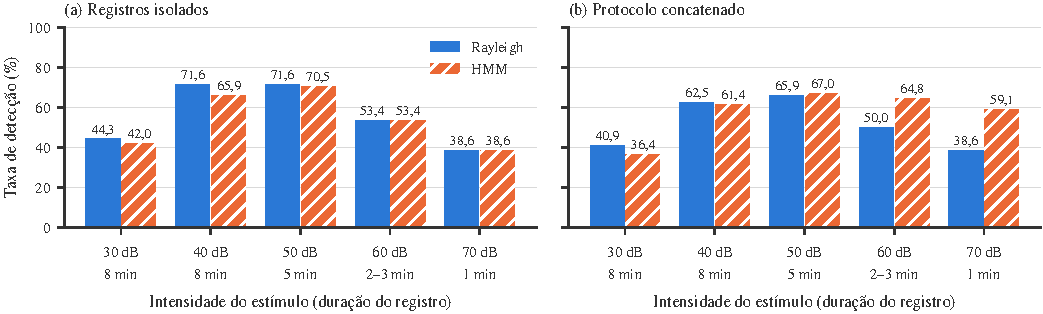
\includegraphics[width=0.8\textwidth]{figuras/fig_deteccao_pt.pdf}
\caption{Taxa de detecção por intensidade do estímulo, deixando um participante de fora. (a) Cada registro analisado como um exame independente. (b) Registros de cada participante analisados como uma única sequência, da ausência de estímulo até 70 dB. A duração do registro é mostrada abaixo de cada intensidade.}
\label{fig:deteccao}
\end{figure*}

\subsection{Calibração e validação}

A densidade Ausente \eqref{eq:aus} foi ajustada por máxima verossimilhança aos valores de $Z$ dos registros sem estimulação. O modelo Presente \eqref{eq:hier} foi calibrado com as sequências de $Z$ de todos os registros com estimulação: como todos os participantes têm audição normal, todos foram contados como resposta presente.

Os valores de $\pi$, $A$ e a regra de parada foram escolhidos por busca em grade (12 valores de $\pi$, 12 e 9 valores para as duas probabilidades de transição, 144 regras), maximizando a taxa de detecção sujeita a uma taxa de FP nas frequências vizinhas não superior à do detector de referência. A referência é o teste de Rayleigh com $\alpha=0{,}05$ e detecção após três testes significativos consecutivos.

A validação deixou um participante de fora por vez. Em cada uma das onze rodadas, as densidades, $\pi$, $A$, a regra de parada e o limite de FP foram obtidos apenas a partir dos outros dez participantes e então aplicados ao participante deixado de fora.

\subsection{Experimentos e medidas de desempenho}

Foram realizados quatro experimentos. (i) \textit{Métodos isolados}: o HMM é comparado com o detector de referência, sendo cada método um exame. (ii) \textit{Densidade fixa}: a validação é repetida substituindo \eqref{eq:pred} por uma única densidade Gama ajustada por máxima verossimilhança a todas as sequências de calibração, para medir o que o modelo bayesiano acrescenta. (iii) \textit{Blocos independentes}: a estatística $Z$ é calculada em blocos disjuntos de $M=30$ ou $M=10$ épocas, sem acumular, mantendo as mesmas densidades calibradas no $Z$ acumulado (avaliadas em $N=M$) e comparando o HMM com o teste de Rayleigh em blocos otimizado sob o mesmo limite de FP. (iv) \textit{Protocolo concatenado}: os dados de um participante são analisados, para cada frequência, como uma única sequência na ordem sem estímulo, 30, 40, 50, 60 e 70 dB. A estatística $Z$ reinicia a cada intensidade para ambos os detectores, mas o HMM mantém seu estado de uma intensidade para a seguinte.

A taxa de detecção é a proporção de exames com estimulação nos quais uma resposta foi detectada, e o tempo de detecção é o número de épocas coletadas até a detecção. As taxas de detecção e de FP de dois detectores foram comparadas com o teste exato de McNemar, e os tempos de detecção com o teste de postos sinalizados de Wilcoxon nos exames detectados por ambos.

\section{Resultados}

Todas as taxas desta seção foram obtidas deixando um participante de fora na calibração, como descrito na seção anterior, assim nenhum participante é avaliado com parâmetros ajustados aos seus próprios dados. 

Primeiro são apresentadas as densidades estimadas, que definem o modelo de observação do HMM. Em seguida, o desempenho de cada modelo, que é a comparação principal, e, por fim, as três variações: densidade fixa, blocos independentes e protocolo concatenado.

\subsection{Densidades estimadas}

A densidade Ausente ajustada aos registros sem estimulação ($k_0=0{,}91$, $\mu_0=0{,}87$) é próxima da exponencial teórica. No modelo Presente, as cadeias concordaram ($\hat{R}\le1{,}002$ para os hiperparâmetros em todas as rodadas; ver Apêndice~\ref{app:mcmc}). Apenas para visualização, utilizando todos os participantes, as médias e os desvios padrão \textit{a posteriori} foram $a_k=1{,}46\pm0{,}11$, $b_k=0{,}32\pm0{,}03$, $a_\rho=0{,}29\pm0{,}02$ e $b_\rho=9{,}5\pm1{,}1$.

A Fig.~\ref{fig:emissoes} mostra as densidades resultantes. Como muitos registros estimulados têm resposta fraca, a densidade Presente mantém grande parte de sua massa na mesma região da Ausente, e difere principalmente por uma cauda longa que cresce com $N$. A razão entre as duas densidades é a evidência que uma observação traz. Com $N=120$, um valor $Z=6$ é 20 vezes mais provável sob Presente, enquanto $Z=1$ é quase neutro (1,1). Após 480 épocas, um valor baixo como $Z=0{,}5$ passa a ser evidência de ausência, sendo 3,4 vezes mais provável sob Ausente.

\begin{table}[t]
\caption{Desempenho dos detectores, deixando um participante de fora}
\label{tab:geral}
\centering
\setlength{\tabcolsep}{3.5pt}
\begin{tabular}{@{}lcccc@{}}
\toprule
 & Taxa de & \multicolumn{2}{c}{Falsos positivos} & Tempo (s) \\
\cmidrule(lr){3-4}
Detector & detecção & Vizinhas & Sem estim. & média / mediana \\
\midrule
\multicolumn{5}{@{}l}{\textit{Registros isolados ($Z$ acumulado)}}\\
Rayleigh (ref.) & \textbf{55,9\%} & 8,5\% & \textbf{3,4\%} & 133 / 95 \\
HMM, fixo & 54,5\% & 8,3\% & 6,8\% & 127 / 90 \\
HMM, bayesiano & 54,1\% & 8,3\% & 6,8\% & \textbf{125} / \textbf{80} \\
\midrule
\multicolumn{5}{@{}l}{\textit{Blocos independentes ($M=30$)}}\\
Rayleigh & 30,2\% & 9,5\% & 12,5\% & \textbf{56} / \textbf{30} \\
HMM, bayesiano & \textbf{42,5\%} & 9,5\% & \textbf{2,3\%} & 126 / 90 \\
\midrule
\multicolumn{5}{@{}l}{\textit{Blocos independentes ($M=10$)}}\\
Rayleigh & \textbf{19,8\%} & \textbf{8,9\%} & 9,1\% & \textbf{63} / \textbf{50} \\
HMM, bayesiano & 19,1\% & 9,1\% & \textbf{4,5\%} & 181 / 150 \\
\midrule
\multicolumn{5}{@{}l}{\textit{Protocolo concatenado}}\\
Rayleigh & 51,6\% & \textbf{6,1\%} & 5,7\% & 125 / 80 \\
HMM & \textbf{57,7\%} & 8,0\% & \textbf{2,3\%} & \textbf{101} / \textbf{30} \\
\bottomrule
\end{tabular}
\end{table}

\subsection{Registros isolados}

A Tabela~\ref{tab:geral} apresenta o desempenho dos detectores. O HMM detectou 54,1\% das respostas e o teste de Rayleigh 55,9\%. Em 14 exames somente o teste de Rayleigh detectou a resposta e em 6 somente o HMM, uma diferença que não é significativa ($p=0{,}12$). A taxa de FP nas frequências vizinhas foi praticamente a mesma (8,3\% e 8,5\%, $p=1{,}00$). Nos registros sem estimulação o HMM teve 6,8\% contra 3,4\%, o que corresponde a três exames e também não é significativo ($p=0{,}25$). A mediana do tempo de detecção foi 80 s para o HMM e 95 s para o teste de Rayleigh. Essa diferença por maior que seja, não foi significativa ($p=0{,}68$).

A Fig.~\ref{fig:deteccao}(a) separa a taxa de detecção por intensidade. Os dois detectores seguem o mesmo perfil: a taxa sobe de 30 a 50 dB e cai a 60 e 70 dB, cujos registros são muito mais curtos e dão ao teste sequencial menos oportunidades de detectar. A única diferença visível ocorre a 40 dB.

% A busca escolheu parâmetros semelhantes em todas as rodadas: probabilidade inicial do estado Presente entre 0,1 e 0,3 e, em dez das onze rodadas, uma probabilidade de retorno de Presente para Ausente de 0,5, o maior valor da grade.

\subsection{Densidade fixa}

Substituir a densidade bayesiana por uma única Gama ($k$ entre 0,81 e 0,90 e $\rho$ entre 0,010 e 0,013 ao longo das rodadas) não alterou o desempenho (Tabela~\ref{tab:geral}). As duas versões discordaram em apenas 8 dos 440 exames com estimulação ($p=0{,}73$), tiveram as mesmas taxas de FP e uma diferença  de 2 segundos em média, que não foi significativa ($p=0{,}34$).

\subsection{Blocos independentes}

Quando $Z$ é calculado em blocos disjuntos sem acumulação (Tabela~\ref{tab:geral}), a detecção cai fortemente em relação ao teste acumulado. Com $M=30$ épocas por bloco, o HMM superou o teste de Rayleigh em blocos (42,5\% contra 30,2\%, $p<0{,}001$), mantendo a mesma taxa de FP nas frequências vizinhas (9,5\%, $p=1{,}00$) e reduzindo o FP nos registros sem estimulação (2,3\% contra 12,5\%, $p=0{,}01$), com maior tempo de detecção (mediana de 90 s contra 30 s). Com $M=10$, ambos caíram para cerca de 19\% ($p=0{,}85$), pois blocos tão curtos dificilmente separam respostas fracas do ruído.

\subsection{Protocolo concatenado}

Quando os registros foram analisados como uma única sequência, o HMM detectou 57,7\% das respostas contra 51,6\% do teste de Rayleigh ($p=0{,}005$). A Fig.~\ref{fig:deteccao}(b) mostra que o ganho se concentra nos registros curtos: 64,8\% contra 50,0\% a 60 dB e 59,1\% contra 38,6\% a 70 dB. A 30 dB, o primeiro registro com estimulação, o HMM detectou menos (36,4\% contra 40,9\%).

A taxa de FP nas frequências vizinhas foi numericamente maior para o HMM (8,0\% contra 6,1\%), mas a diferença não foi significativa ($p=0{,}16$). Por outro lado, a 70 dB, 44 das 52 detecções do HMM ocorreram na primeira avaliação permitida, 30 s após o início do registro. Essas detecções são herdadas do estado alcançado a 60 dB mais do que sustentadas por dados novos.

\section{Discussão e conclusões}

Com cada registro tratado como um exame, o HMM não melhorou o teste de Rayleigh: taxa de detecção, taxa de FP e tempo de detecção foram estatisticamente iguais. O resultado provavelmente é explicado pelo ORD escolhido, a estatística acumulada já resume todas as épocas coletadas, de modo que $Z_{20}$ contém as épocas de $Z_{10}$. As observações estão longe de ser independentes dado o estado, como o HMM supõe, e a sequência tem pouco a acrescentar ao seu último valor. Os parâmetros selecionados apontam na mesma direção: com probabilidade de 0,5 de sair do estado Presente, o modelo quase não guarda memória, e sua decisão se aproxima de uma comparação do último $Z$ com um limiar que depende de $N$. O experimento em blocos independentes confirma essa interpretação: com $M=30$, o HMM supera o teste de Rayleigh em blocos ao acumular evidência entre janelas, mas ainda fica abaixo do teste acumulado porque descartar a coerência de fase entre blocos reduz o poder estatístico.

Outro ponto, é que a igualdade entre a densidade bayesiana e a fixa indica que a detecção é limitada pela informação contida em $Z$, e não pelo nível de detalhe com que sua distribuição é descrita.

O protocolo concatenado mostra onde o o uso de HMM ajuda, uma resposta encontrada em uma intensidade torna mais provável uma resposta na intensidade seguinte, e esse é é o principal achado desse trabalho. O HMM a utilizou para detectar mais cedo e com mais frequência em registros curtos demais para o teste de Rayleigh. A mesma memória, porém, pode carregar erros adiante, o que apareceu como uma taxa de FP numericamente mais alta, embora sem diferença significativa.

Esses dois comportamentos não são exclusivos do teste de Rayleigh. O Apêndice~\ref{app:ords} repete a validação com outros quatro ORDs como observação: MSC, $T^2$ de Hotelling, coerência múltipla e teste F espectral. Com registros isolados, o HMM também não melhorou nenhum deles. No protocolo concatenado, melhorou todos, e a maior taxa de detecção foi obtida com o $T^2$ de Hotelling (64,1\%).

Em resumo, os resultados deste estudo demonstram que substituir o valor crítico de um teste de Rayleigh sequencial por um HMM não melhora a detecção da ASSR quando a observação é a própria estatística, com ou sem um ajuste bayesiano. O HMM torna-se vantajoso quando o exame é visto como uma sequência de registros, sem aumento significativo de falsos positivos. 

\bibliographystyle{IEEEtran}
\bibliography{reference}

\clearpage
\appendices
\section{Diagnóstico de convergência do MCMC por rodada de validação}
\label{app:mcmc}

Este apêndice apresenta os diagnósticos de convergência do amostrador Metropolis e Gibbs utilizado para estimar os quatro hiperparâmetros do modelo do estado Presente ($a_k$, $b_k$, $a_\rho$ e $b_\rho$) em cada uma das onze rodadas da validação deixando um participante de fora. Em cada rodada, o modelo é calibrado com os dez participantes restantes por meio de quatro cadeias independentes de 20\,000 iterações, com descarte inicial (\textit{burn-in}) de 5\,000 iterações e subamostragem (\textit{thinning}) a cada 10 iterações, totalizando 6\,000 amostras agrupadas \textit{a posteriori}.

A Tabela~\ref{tab:mcmc_loso} resume, para cada participante deixado de fora, a média e o desvio padrão \textit{a posteriori} de cada hiperparâmetro, o maior valor da estatística $\hat{R}$ de Gelman--Rubin dividido \cite{gelman1992,gelman2013}, o menor tamanho efetivo de amostra (ESS, calculado após a subamostragem) e a taxa média de aceitação dos passos de Metropolis nos hiperparâmetros. Em todas as rodadas e para todos os hiperparâmetros, observa-se $\hat{R} \le 1{,}002$ e $\mathrm{ESS} \ge 2\,047$, indicando mistura adequada e convergência das cadeias.

As Figs.~\ref{fig:mcmc_Ab} a~\ref{fig:mcmc_Wr} detalham visualmente cada uma das onze rodadas. Cada figura é organizada em uma grade $3 \times 4$ (uma coluna por hiperparâmetro): a primeira linha exibe as trajetórias das quatro cadeias (com o fim do \textit{burn-in} destacado e o valor de $\hat{R}$ anotado); a segunda linha mostra a função de autocorrelação média pós-\textit{burn-in} (com a defasagem de subamostragem e o ESS anotados); e a terceira linha apresenta o histograma da distribuição \textit{a posteriori} resultante (com a média e $\pm 1$ desvio padrão indicados).

\begin{table*}[t]
\caption{Resumo das estimativas \textit{a posteriori} e dos critérios de convergência do MCMC em cada rodada de validação (participante deixado de fora).}
\label{tab:mcmc_loso}
\centering
\begin{tabular}{@{}lccccccc@{}}
\toprule
Participante & $a_k$ & $b_k$ & $a_\rho$ & $b_\rho$ & $\hat{R}_{\max}$ & $\mathrm{ESS}_{\min}$ & Aceitação \\
\midrule
Ab & $1{,}41 \pm 0{,}11$ & $0{,}30 \pm 0{,}03$ & $0{,}28 \pm 0{,}02$ & $8{,}8 \pm 1{,}1$ & 1,000 & 2\,243 & 0,45 \\
An & $1{,}50 \pm 0{,}12$ & $0{,}35 \pm 0{,}03$ & $0{,}28 \pm 0{,}02$ & $9{,}6 \pm 1{,}2$ & 1,002 & 2\,047 & 0,44 \\
Bb & $1{,}47 \pm 0{,}11$ & $0{,}32 \pm 0{,}03$ & $0{,}31 \pm 0{,}02$ & $10{,}2 \pm 1{,}2$ & 1,001 & 2\,334 & 0,44 \\
Er & $1{,}44 \pm 0{,}11$ & $0{,}31 \pm 0{,}03$ & $0{,}27 \pm 0{,}02$ & $8{,}7 \pm 1{,}1$ & 1,001 & 2\,149 & 0,45 \\
Lu & $1{,}46 \pm 0{,}11$ & $0{,}32 \pm 0{,}03$ & $0{,}30 \pm 0{,}02$ & $9{,}3 \pm 1{,}1$ & 1,001 & 2\,170 & 0,44 \\
Qu & $1{,}46 \pm 0{,}11$ & $0{,}32 \pm 0{,}03$ & $0{,}28 \pm 0{,}02$ & $8{,}8 \pm 1{,}1$ & 1,000 & 2\,082 & 0,44 \\
Sa & $1{,}58 \pm 0{,}12$ & $0{,}38 \pm 0{,}04$ & $0{,}31 \pm 0{,}02$ & $13{,}7 \pm 1{,}7$ & 1,001 & 2\,071 & 0,44 \\
So & $1{,}46 \pm 0{,}11$ & $0{,}32 \pm 0{,}03$ & $0{,}28 \pm 0{,}02$ & $8{,}8 \pm 1{,}1$ & 1,001 & 2\,107 & 0,45 \\
Ti & $1{,}44 \pm 0{,}11$ & $0{,}30 \pm 0{,}03$ & $0{,}31 \pm 0{,}02$ & $9{,}5 \pm 1{,}1$ & 1,001 & 2\,096 & 0,44 \\
Vi & $1{,}42 \pm 0{,}11$ & $0{,}29 \pm 0{,}03$ & $0{,}31 \pm 0{,}02$ & $9{,}3 \pm 1{,}1$ & 1,001 & 2\,147 & 0,44 \\
Wr & $1{,}45 \pm 0{,}11$ & $0{,}31 \pm 0{,}03$ & $0{,}28 \pm 0{,}02$ & $9{,}1 \pm 1{,}1$ & 1,002 & 2\,162 & 0,44 \\
\bottomrule
\end{tabular}
\end{table*}

\begin{figure*}[t]
\centering
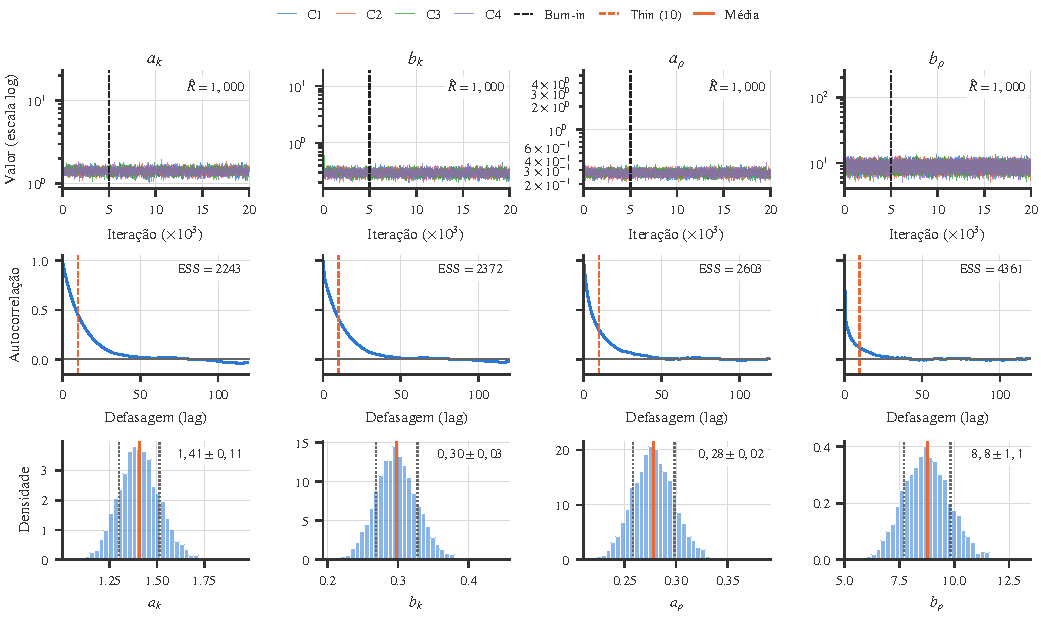
\includegraphics[width=\textwidth]{figuras/fig_mcmc_Ab_pt.pdf}
\caption{Diagnóstico MCMC da rodada com o participante Ab deixado de fora ($\hat{R}_{\max}=1{,}000$; $\mathrm{ESS}_{\min}=2\,243$): trajetórias das quatro cadeias, autocorrelação pós-\textit{burn-in} e distribuição \textit{a posteriori} dos hiperparâmetros $a_k$, $b_k$, $a_\rho$ e $b_\rho$.}
\label{fig:mcmc_Ab}
\end{figure*}

\begin{figure*}[t]
\centering
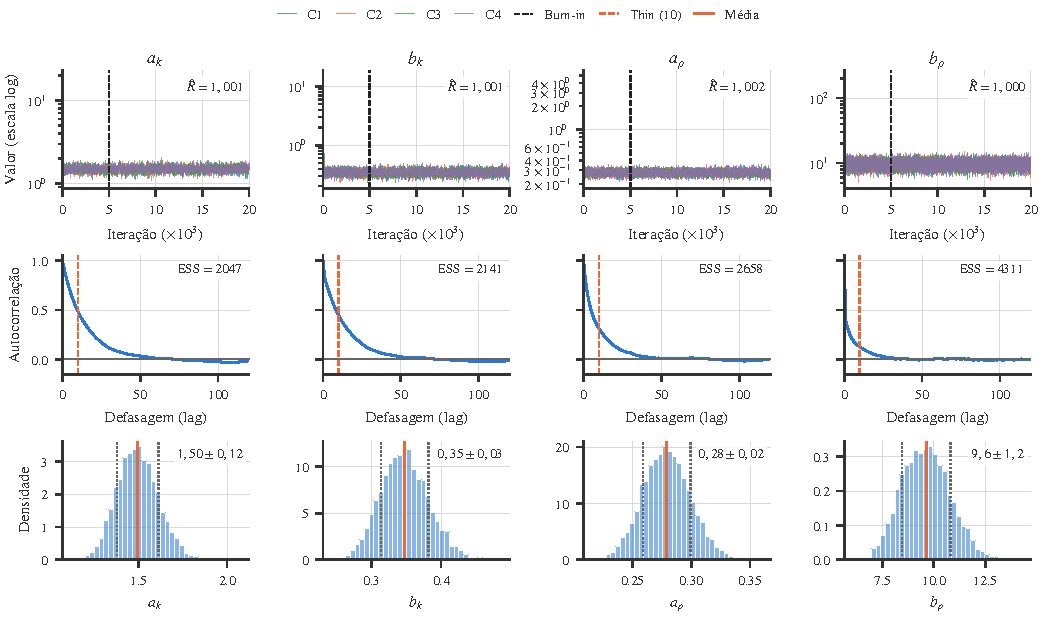
\includegraphics[width=\textwidth]{figuras/fig_mcmc_An_pt.pdf}
\caption{Diagnóstico MCMC da rodada com o participante An deixado de fora ($\hat{R}_{\max}=1{,}002$; $\mathrm{ESS}_{\min}=2\,047$): trajetórias das quatro cadeias, autocorrelação pós-\textit{burn-in} e distribuição \textit{a posteriori} dos hiperparâmetros $a_k$, $b_k$, $a_\rho$ e $b_\rho$.}
\label{fig:mcmc_An}
\end{figure*}

\begin{figure*}[t]
\centering
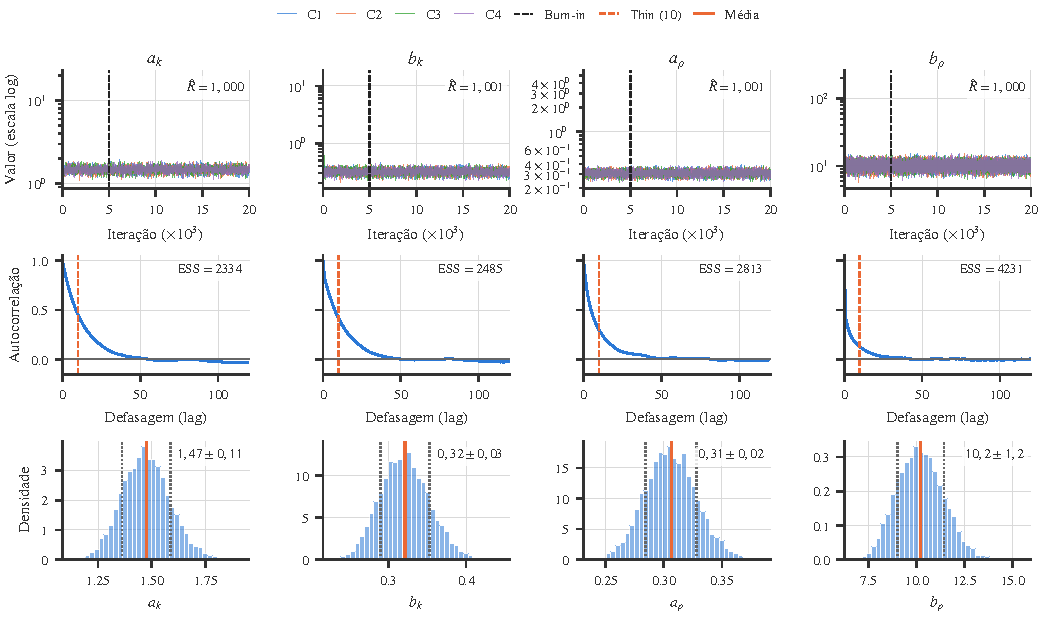
\includegraphics[width=\textwidth]{figuras/fig_mcmc_Bb_pt.pdf}
\caption{Diagnóstico MCMC da rodada com o participante Bb deixado de fora ($\hat{R}_{\max}=1{,}001$; $\mathrm{ESS}_{\min}=2\,334$): trajetórias das quatro cadeias, autocorrelação pós-\textit{burn-in} e distribuição \textit{a posteriori} dos hiperparâmetros $a_k$, $b_k$, $a_\rho$ e $b_\rho$.}
\label{fig:mcmc_Bb}
\end{figure*}

\begin{figure*}[t]
\centering
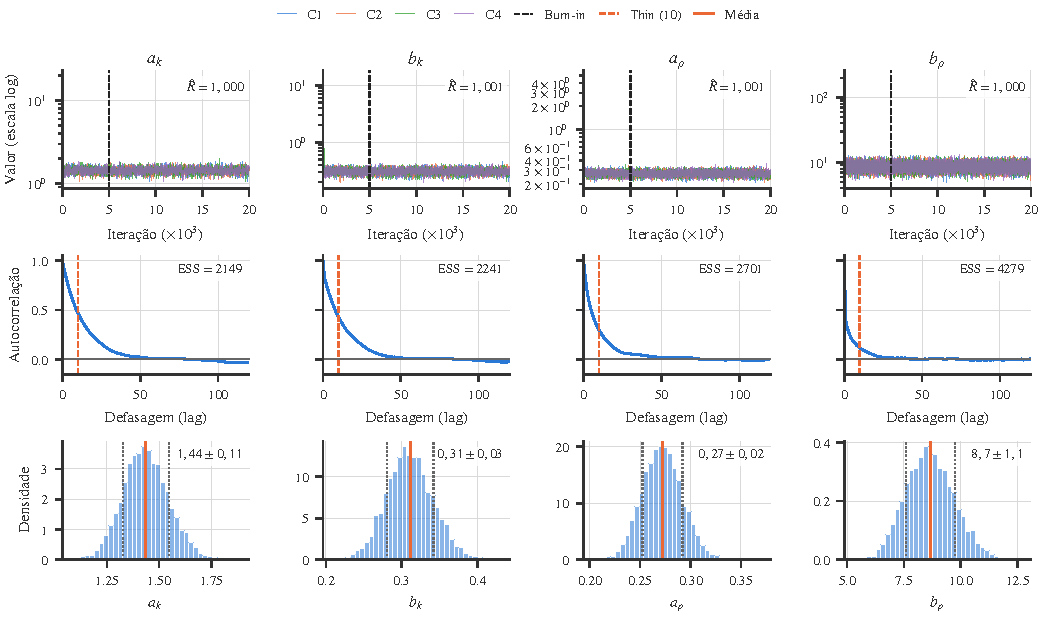
\includegraphics[width=\textwidth]{figuras/fig_mcmc_Er_pt.pdf}
\caption{Diagnóstico MCMC da rodada com o participante Er deixado de fora ($\hat{R}_{\max}=1{,}001$; $\mathrm{ESS}_{\min}=2\,149$): trajetórias das quatro cadeias, autocorrelação pós-\textit{burn-in} e distribuição \textit{a posteriori} dos hiperparâmetros $a_k$, $b_k$, $a_\rho$ e $b_\rho$.}
\label{fig:mcmc_Er}
\end{figure*}

\begin{figure*}[t]
\centering
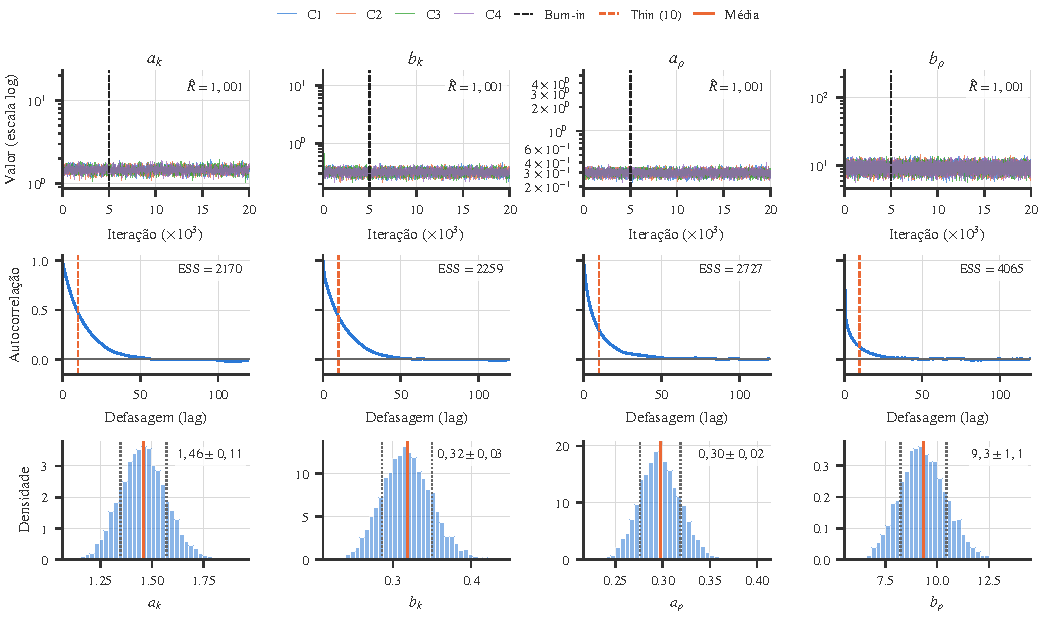
\includegraphics[width=\textwidth]{figuras/fig_mcmc_Lu_pt.pdf}
\caption{Diagnóstico MCMC da rodada com o participante Lu deixado de fora ($\hat{R}_{\max}=1{,}001$; $\mathrm{ESS}_{\min}=2\,170$): trajetórias das quatro cadeias, autocorrelação pós-\textit{burn-in} e distribuição \textit{a posteriori} dos hiperparâmetros $a_k$, $b_k$, $a_\rho$ e $b_\rho$.}
\label{fig:mcmc_Lu}
\end{figure*}

\begin{figure*}[t]
\centering
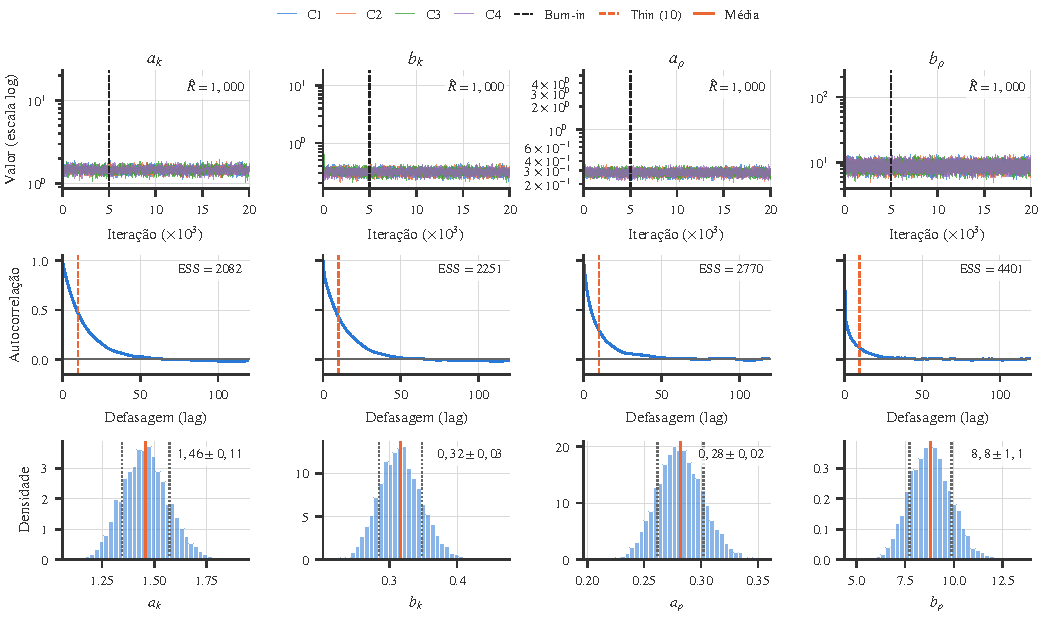
\includegraphics[width=\textwidth]{figuras/fig_mcmc_Qu_pt.pdf}
\caption{Diagnóstico MCMC da rodada com o participante Qu deixado de fora ($\hat{R}_{\max}=1{,}000$; $\mathrm{ESS}_{\min}=2\,082$): trajetórias das quatro cadeias, autocorrelação pós-\textit{burn-in} e distribuição \textit{a posteriori} dos hiperparâmetros $a_k$, $b_k$, $a_\rho$ e $b_\rho$.}
\label{fig:mcmc_Qu}
\end{figure*}

\begin{figure*}[t]
\centering
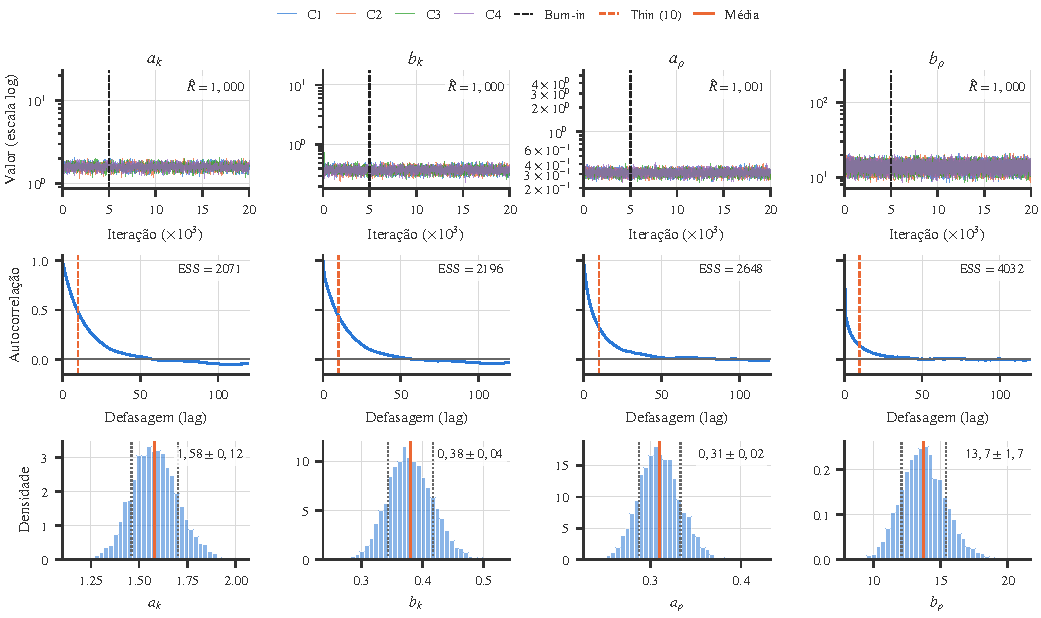
\includegraphics[width=\textwidth]{figuras/fig_mcmc_Sa_pt.pdf}
\caption{Diagnóstico MCMC da rodada com o participante Sa deixado de fora ($\hat{R}_{\max}=1{,}001$; $\mathrm{ESS}_{\min}=2\,071$): trajetórias das quatro cadeias, autocorrelação pós-\textit{burn-in} e distribuição \textit{a posteriori} dos hiperparâmetros $a_k$, $b_k$, $a_\rho$ e $b_\rho$.}
\label{fig:mcmc_Sa}
\end{figure*}

\begin{figure*}[t]
\centering
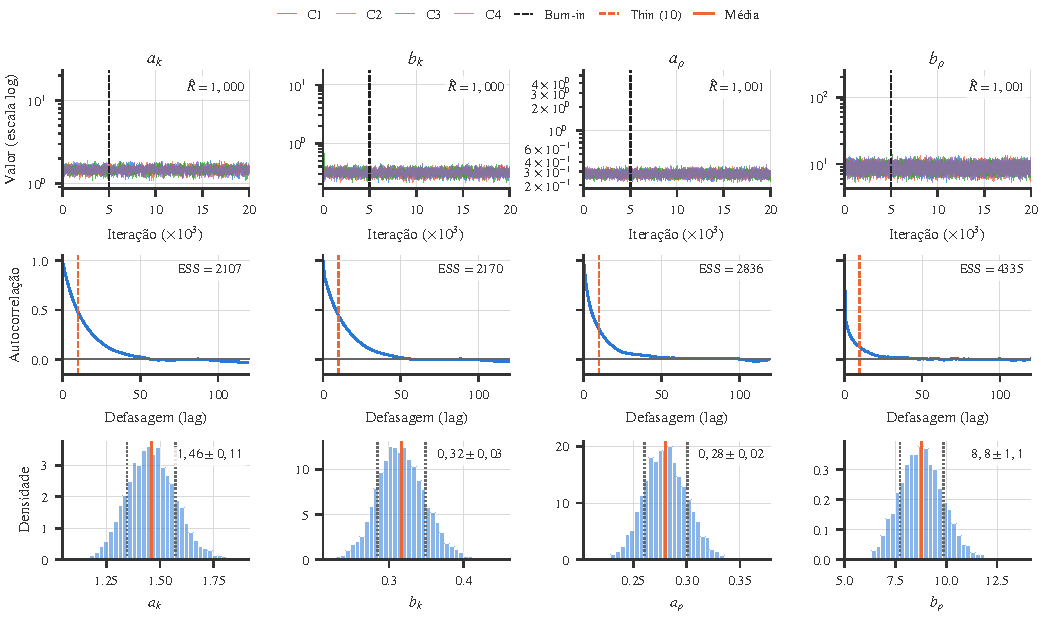
\includegraphics[width=\textwidth]{figuras/fig_mcmc_So_pt.pdf}
\caption{Diagnóstico MCMC da rodada com o participante So deixado de fora ($\hat{R}_{\max}=1{,}001$; $\mathrm{ESS}_{\min}=2\,107$): trajetórias das quatro cadeias, autocorrelação pós-\textit{burn-in} e distribuição \textit{a posteriori} dos hiperparâmetros $a_k$, $b_k$, $a_\rho$ e $b_\rho$.}
\label{fig:mcmc_So}
\end{figure*}

\begin{figure*}[t]
\centering
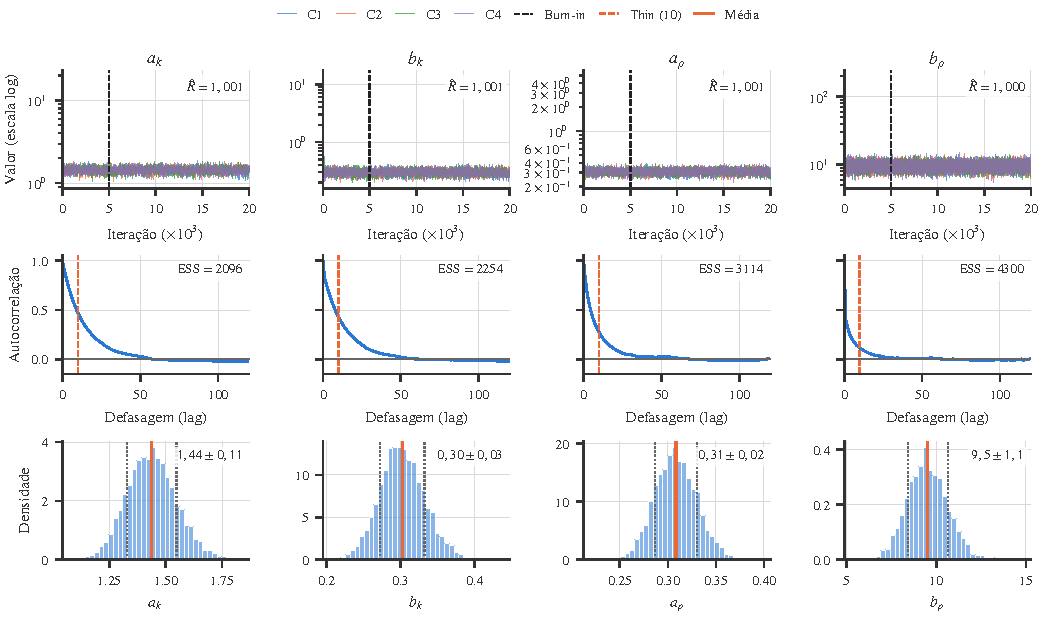
\includegraphics[width=\textwidth]{figuras/fig_mcmc_Ti_pt.pdf}
\caption{Diagnóstico MCMC da rodada com o participante Ti deixado de fora ($\hat{R}_{\max}=1{,}001$; $\mathrm{ESS}_{\min}=2\,096$): trajetórias das quatro cadeias, autocorrelação pós-\textit{burn-in} e distribuição \textit{a posteriori} dos hiperparâmetros $a_k$, $b_k$, $a_\rho$ e $b_\rho$.}
\label{fig:mcmc_Ti}
\end{figure*}

\begin{figure*}[t]
\centering
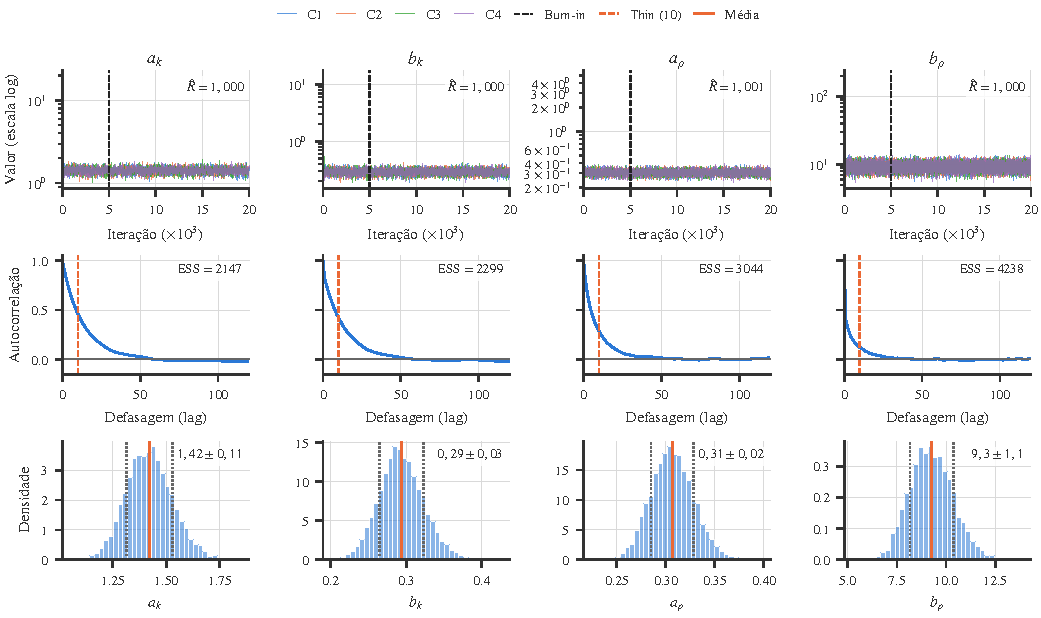
\includegraphics[width=\textwidth]{figuras/fig_mcmc_Vi_pt.pdf}
\caption{Diagnóstico MCMC da rodada com o participante Vi deixado de fora ($\hat{R}_{\max}=1{,}001$; $\mathrm{ESS}_{\min}=2\,147$): trajetórias das quatro cadeias, autocorrelação pós-\textit{burn-in} e distribuição \textit{a posteriori} dos hiperparâmetros $a_k$, $b_k$, $a_\rho$ e $b_\rho$.}
\label{fig:mcmc_Vi}
\end{figure*}

\begin{figure*}[t]
\centering
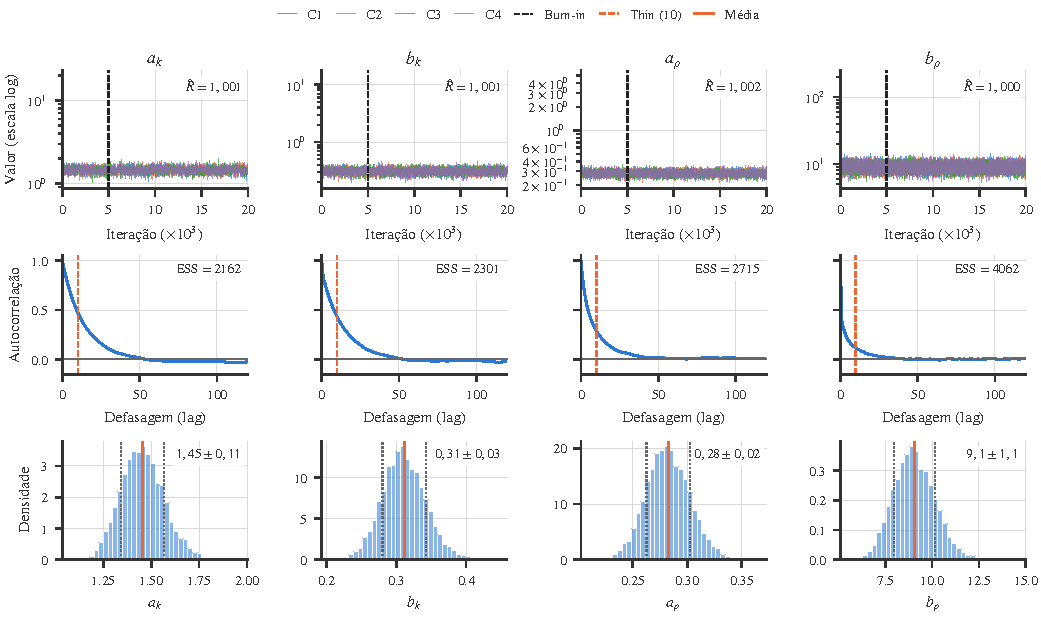
\includegraphics[width=\textwidth]{figuras/fig_mcmc_Wr_pt.pdf}
\caption{Diagnóstico MCMC da rodada com o participante Wr deixado de fora ($\hat{R}_{\max}=1{,}002$; $\mathrm{ESS}_{\min}=2\,162$): trajetórias das quatro cadeias, autocorrelação pós-\textit{burn-in} e distribuição \textit{a posteriori} dos hiperparâmetros $a_k$, $b_k$, $a_\rho$ e $b_\rho$.}
\label{fig:mcmc_Wr}
\end{figure*}

\clearpage
\section{Ablação: outros ORDs como observação}
\label{app:ords}


\begin{table*}[h]
\caption{Desempenho do HMM com cada ORD como observação, deixando um participante de fora. Entre parênteses, a diferença em relação ao mesmo ORD sem HMM (pontos percentuais; segundos no tempo).}
\label{tab:ords}
\centering
\begin{tabular}{@{}lcccc@{}}
\toprule
 & Taxa de & \multicolumn{2}{c}{Falsos positivos} & Tempo (s) \\
\cmidrule(lr){3-4}
Observação & detecção & Vizinhas & Sem estim. & média / mediana \\
\midrule
\multicolumn{5}{@{}l}{\textit{Métodos isolados}}\\
Rayleigh & 54,1\% ($-$1,4) & 8,3\% ($-$0,6) & 6,8\% (+3,4) & 125 / 80 ($-$7 / $-$10) \\
MSC & 56,4\% ($-$2,2) & 10,2\% (+1,7) & 5,7\% ($-$3,4) & 122 / 80 ($-$2 / 0) \\
$T^2$ de Hotelling & 55,2\% ($-$2,8) & 8,7\% (+1,3) & 5,7\% ($-$3,4) & 125 / 80 (+6 / +10) \\
MMSC (4 eletrodos) & 44,1\% (+0,2) & 9,5\% (+0,4) & 3,4\% (0,0) & 151 / 130 (+3 / +10) \\
F espectral & 54,3\% ($-$1,2) & 9,1\% (+0,2) & 3,4\% ($-$1,1) & 135 / 90 (+6 / +10) \\
\midrule
\multicolumn{5}{@{}l}{\textit{Protocolo concatenado}}\\
Rayleigh & 57,7\% (+6,1) & 8,0\% (+1,9) & 2,3\% ($-$3,4) & 101 / 30 ($-$24 / $-$50) \\
MSC & 63,2\% (+10,2) & 6,2\% (+0,5) & 2,3\% ($-$2,2) & 96 / 30 ($-$48 / $-$70) \\
$T^2$ de Hotelling & \textbf{64,1\%} (+13,2) & 7,2\% (0,0) & 1,1\% ($-$5,7) & 93 / 30 ($-$30 / $-$50) \\
MMSC (4 eletrodos) & 58,4\% (+17,3) & 7,6\% (+0,8) & 2,3\% ($-$3,4) & 86 / 30 ($-$56 / $-$80) \\
F espectral & 56,8\% (+7,7) & 7,6\% (+1,0) & 1,1\% (0,0) & 90 / 30 ($-$41 / $-$60) \\
\bottomrule
\end{tabular}
\end{table*}


Qualquer ORD pode ser a observação do HMM: calcula-se o valor-p do teste a cada avaliação e usa-se $Z=-\ln p$. Para o teste de Rayleigh, isso devolve a própria estatística \eqref{eq:z}; para os demais, sem resposta, $Z$ segue uma exponencial de média um, como $Z_N$. Assim, as densidades e o HMM não mudam. Foram testados quatro ORDs, todos acumulados desde o início do registro ($X_i$ é o coeficiente de Fourier da época $i$):

\begin{itemize}
\item \textit{Coerência quadrática de magnitude} (MSC), no eletrodo FC: $\mathrm{MSC}_N=\big|\sum_i X_i\big|^2\big/\big(N\sum_i|X_i|^2\big)$. Sem resposta, $\mathrm{MSC}_N\sim\mathrm{Beta}(1,N-1)$ e $p=(1-\mathrm{MSC}_N)^{N-1}$. Ao contrário do teste de Rayleigh, usa a fase e a amplitude.
\item \textit{$T^2$ de Hotelling}, no eletrodo FC: testa se a média dos pontos $(\mathrm{Re}\,X_i,\mathrm{Im}\,X_i)$ é nula, com a matriz de covariância $2\times2$ completa. Sem resposta, $\frac{N-2}{2(N-1)}T^2\sim F(2,N-2)$.
\item \textit{Coerência múltipla} (MMSC), nos eletrodos FC, Fz, Cz e F4 ($L=4$): com $\mathbf{Y}_i\in\mathbb{C}^L$ os coeficientes dos $L$ eletrodos, $\mathbf{V}=\sum_i\mathbf{Y}_i$ e $\mathbf{S}=\sum_i\mathbf{Y}_i\mathbf{Y}_i^{H}$, $\kappa^2_N=\mathbf{V}^{H}\mathbf{S}^{-1}\mathbf{V}/N$. Sem resposta, $\kappa^2_N\sim\mathrm{Beta}(L,N-L)$.
\item \textit{Teste F espectral}, no eletrodo FC: $F=N\,|\bar{X}|^2$ dividido pela potência média por época em 20 frequências vizinhas sem estímulo. Sem resposta, $F\sim F(2,40N)$. Como as frequências de modulação e as frequências vizinhas usadas para medir FP se alternam a cada 1 Hz entre 81 e 96 Hz, as frequências de ruído foram tomadas fora dessa faixa, de 70 a 79 Hz e de 98 a 107 Hz.
\end{itemize}

O restante da validação é o do texto principal, inclusive o limite de FP e o modelo Presente amostrado por MCMC. A Tabela~\ref{tab:ords} compara cada ORD com ele mesmo usado sem HMM.


Com registros isolados, o HMM não melhorou nenhum ORD. No protocolo concatenado, melhorou todos, e o melhor resultado foi com o $T^2$ de Hotelling (64,1\%, contra 57,7\% com Rayleigh), sem teste de significância entre ORDs.



\end{document}
